%************************************************
\chapter[Application du modèle à l'évaluation]{Application du modèle morphologique à l'évaluation des algorithmes d'analyse automatique de scènes sonores environnementales}\label{ch:ml_simuperf}
%************************************************

\section{Le challenge DCASE  2013}

\subsection{Objectif}


\subsection{Génération des corpus}

\begin{table}[t]
\begin{center}
\begin{tabular}{lcc}
\textbf{Index} & \textbf{Nom}  & \textbf{Description}  \\ 
\hline
1   & porte-frapper & Frapper à la porte \\
2   & porte-claquer & Claquer la porte \\
3   & parole        & Personne  prononçant \\
    &               &  une phrase \\
4   & rire          & Personne riant  \\    
5   & gorge         & Personne se   \\
    &               & raclant la gorge \\
6   & toux          & Personne toussant \\
7   & tiroir        & Ouverture/fermeture d'un tiroir \\
8   & imprimante    & Bruit d'une imprimante \\
9   & clavier       & Bruit des touches d'un clavier \\
10  & souris        & Bruit d'un clique de souris \\
11  & stylo         & Poser un stylo sur une table \\
12  & bouton        & Bouton permettant d'allumer la lumière \\
13  & clefs         & Poser un jeu de clefs sur une table \\    
14  & téléphone     & Sonnerie de téléphone \\
15  & alerte        & bruit d'une alerte \\
    &               & électronique  (ordinateur, mobile) \\
16  & page          & Tourner une page \\     
\hline      
\end{tabular}
\end{center}
\label{tab:eventDCASE2013}
\caption{Les 16 classes de sons utilisées dans le challenge DCASE 2013}
\end{table}

Cette section décrit les différents corpus de scènes simulées utilisées lors de l'expérience. Tous les corpus  de scènes simulées sont générées à partir des scènes enregistrées du corpus \emph{test-QMUL} : le corpus de \emph{test} de la tâche de détection d'événement (AED) du challenge DCASE 2013  \citep{giannoulis2013detection} (\cf~Section~\ref{sec:ch6_dcase2013AED}). 

\emph{test-QMUL} a été enregistré à l'université \emph{Queen Mary University of London}, il est composé de 11 enregistrements d'ambiances de bureau, toutes d'une durée proche de 1 minute. Chaque scène est une séquence  d'événements sonores non enchevêtrés. Ces événements sont repartis en 16 classes de sons, détaillées dans le tableau~\ref{tab:eventDCASE2013}. Les enregistrements ont été effectués dans 5 environnements acoustiques différents. Les scènes sont annotées par deux individus différents. Pour chaque scène et à chaque événement entendu, l'annotateur indique la classe de l'événement, son \emph{onset} et son \emph{offset}.  Toutes les annotations sont utilisées, formant ainsi une vérité terrain composée de 22 couples scène-annotateur.


À partir des annotations de \emph{test-QMUL}, quatre corpus de scènes simulées ont été générés, mettant en œuvre deux banques de données de sons isolées ainsi que deux processus de simulation distincts. Les banques de données de sons isolées et les processus de simulation sont détaillés dans les sections suivantes (\cf~Sections~\ref{sec:ch7_eventDataset},~\ref{sec:ch7_simuProcessInstance} et~\ref{sec:ch7_simuProcessAbstract}). \\

\gl{TODO: définir offset, peut être ailleurs}

\begin{figure}[t]
\begin{center}
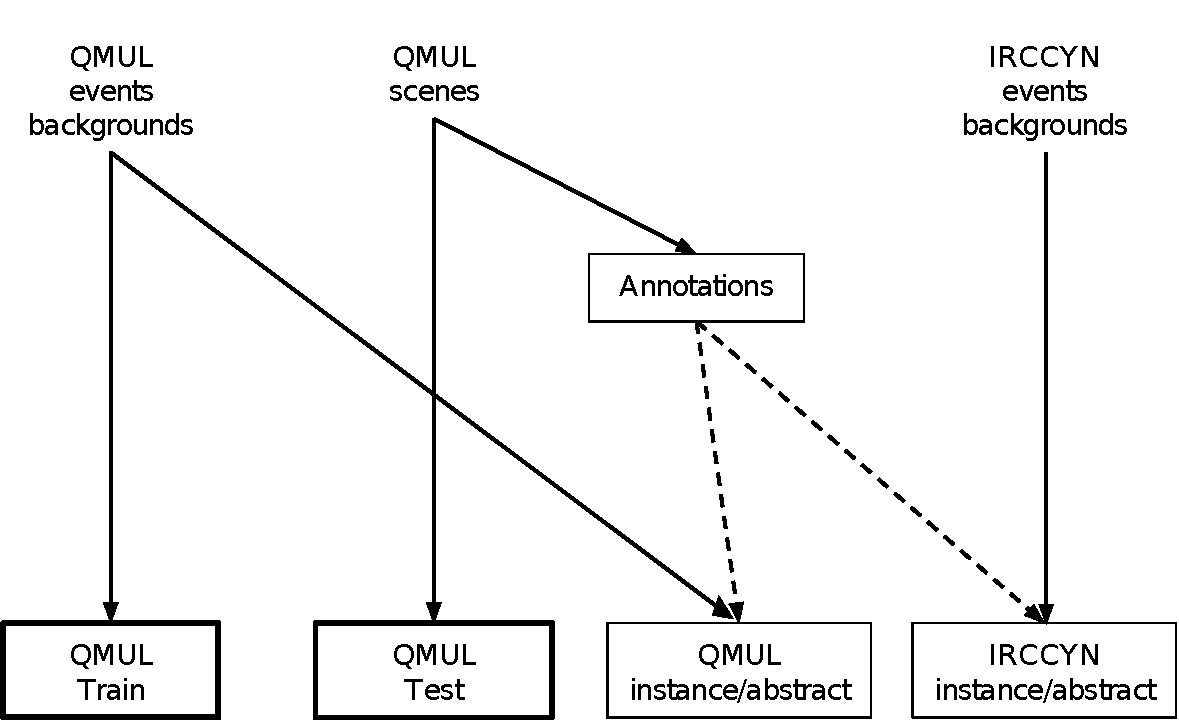
\includegraphics[width=1\textwidth]{gfxML/databasesTasslp.pdf}
\label{fig:databasesDCASE2013Simu}
\caption{Generation process of the corpora considered in this evaluation. As part of the DCASE challenge, systems were trained on QMUL Train and tested on QMUL Test during the DCASE challenge.} 
\end{center}
\end{figure}

\subsubsection{Banque de données de sons isolés \emph{QMUL} et \emph{IRCCYN}}
\label{sec:ch7_eventDataset}

Deux banques de sons isolées sont utilisés pour générer les scènes isolées. Elles sont respectivement nommée \emph{QMUL} et \emph{IRCCYN}. Toutes deux sont composés de deux types de sons:

\begin{itemize}
\item les événements: les enregistrements de sons isolés devant être détectés et identifiés par les algorithmes;
\item les \emph{backgrounds}: les enregistrements de fonds sonores, \ie~des scènes amorphes (textures, \cf~Section~\ref{sec:ch4_eventTextureAmorphe}) ne possédant pas d'événement saillant, qui rendent compte de l’environnement acoustique naturel inhérent au lieu d'occurrence des événements. 
\end{itemize}

Les sons isolés de la banque \emph{QMUL} sont extraits de scènes enregistrées à l'université \emph{Queen Mary University of London} (QMUL) dans le cadre de la préparation du challenge AED DCASE-2013, mais n'ayant pas été utilisées lors de l'évaluation,~\ie ne faisant pas partie des corpus de \emph{test} (\emph{test-QMUL}) et de \emph{development}. Ces sons isolées profitent donc des mêmes conditions d’enregistrement que les scènes du corpus \emph{test-QMUL} \citep{Giannoulis:2013a}. Le nombre d'événements par classe varie de 3 à 23. Les enregistrements de \emph{backgrounds} ont été réalisés sur les mêmes environnements acoustiques que ceux utilisés pour le corpus \emph{test-QMUL}, avec là encore les mêmes conditions d'enregistrements.

La banque \emph{IRCCYN} est une nouvelle banque de sons isolés, enregistrées à l'Institut de Recherche en Cybernétique de Nantes (IRCCyN). Cette dernière comprend les mêmes classes que celles présentes dans le corpus \emph{test-QMUL} (\cf~Tableau~\ref{tab:eventDCASE2013}). Les enregistrement ont été effectués dans un environnement calme, à l'aide d'un micro canon \emph{AT8035} connecté à un enregistreur \emph{ZOOM H4n}. Chaque classe est composée de 20 événements sonores, ce qui correspond au nombre d'événements disponibles dans le corpus de \emph{train} du AED DCASE-2013 \citep{Giannoulis:2013a}. Les \emph{background} ont été enregistrés de nuit, dans les bureaux de l'IRCCyN, afin qu'ils ne soient pas pollués par des bruits non souhaités. \\

\gl{TODO: détailler la banque de données IRCCYN}

\subsubsection{Processus de simulation \emph{instance}}
\label{sec:ch7_simuProcessInstance}

Pour le processus de simulation \emph{instance}, l'objectif est de générer des scènes simulées qui ressemblent le plus possible aux scènes du corpus \emph{test-QMUL}. Cette ressemblance se comprend suivant deux aspects:

\begin{itemize}
\item \emph{la structure temporelle}: le positionnement temporel en termes d'\emph{onsets} des événements sonores;
\item \emph{les niveaux sonores des événements}: la puissance du ratio entre l'énergie de l'événement et celle du \emph{background}, notée EBR (\emph{event to Background power Ratios}). L'$EBR$ d'un événement de $N$ échantillons est obtenu en calculant le ratio en décibel entre de la valeur efficace (niveau $RMS$, \cf~Section~\ref{sec:ch5_recordDataSet}) du signal (\cf~Equation~\ref{eq:ch7_eq2}) de l'événement ($E_{rms}$) et du \emph{background}  $B_{rms}$):

\begin{equation}
\label{eq:ch7_eq1}
EBR=20log_{10} \left(  \dfrac{E_{rms}}{B_{rms}} \right) 
\end{equation}

\begin{equation}
\label{eq:ch7_eq2}
X_{rms}=\sqrt{\dfrac{1}{N} \sum_{n=1}^{N} x(n)^2}
\end{equation}

$x(n)$ peut être remplacé par $e(n)$ ou $b(n)$, respectivement les valeurs des signaux de l'événement et du \emph{background} en volt à l'échantillon $n$. 
\end{itemize}


Pour chaque événement et chaque couple scène-annotateur du corpus \emph{test-QMUL}, nous extrayons les positions d'\emph{onsets} et d'{offsets} et calculons une approximation de l'$EBR$. Comme il n'est pas possible d'isoler le signal du \emph{background} des scènes de \emph{test-QMUL}, $B_{rms}$ est obtenu à partir des périodes dénuées d'événements. \\
 
\gl{TODO: expliquer comment on supprime le niveau de bruit dans $E_{rms}$} \\

Les positions \emph{onsets} et les $EBRs$ ainsi recouvrés sont utilisés pour simuler un nouveau corpus de scènes: pour chaque scène simulée, à chaque \emph{onset} d'une annotation (couple scène-annotateur), nous plaçons un événement de la même classe, choisi aléatoirement parmi la banque de sons isolé (\emph{QMUL} ou \emph{IRCCYN}). Afin de garantir que les durées des samples sélectionnés ne soient pas trop long par rapport à celles d'origines, ces derniers sont coupés si leur durée est  supérieure à la durée de l'annotation d'au moins $0.5$ secondes.  Les niveaux des événements des scènes simulées sont fixés par rapports aux $EBRs$ calculés sur les scènes enregistrées. 

Le processus de simulation \emph{instance} ne s'appuie donc pas sur le modèle introduit à la section~\ref{sec:ch4_modelForm}.   L'objectif est d’obtenir des scènes simulées possédant des samples différents des scènes enregistrées, mais dont les structures temporelles et les $EBRs$ sont aussi proches que possible de ceux des scènes du corpus \emph{test-QMUL}.

\subsubsection{Processus de simulation \emph{abstract}}
\label{sec:ch7_simuProcessAbstract}

L'objectif de processus de simulation \emph{abstract} est de capturer les paramètres haut niveaux régissant la structure de la scène enregistrer, et de les utiliser afin de régénérer cette dernière. Le processus \emph{abstract} s'appuie sur le modèle introduit à la section~\ref{sec:ch4_modelForm}. Concrètement, le modèle est instancié suivant des paramètres $\mu_i^a$, $\sigma_i^a$, $\mu_i^t$ et $\sigma_i^t$ (\cf~Équation.~\ref{eq:ch4_eq1} et~\ref{eq:ch4_eq2}) estimés sur la scène enregistrée. Pour chaque couple scène-annotateur du corpus  \emph{test-QMUL}, ces paramètres sont estimés à partir de l'annotation ($\mu_i^t$ et $\sigma_i^t$) et du signal ($\mu_i^a$ et $\sigma_i^a$). Les $EBRs$ et les espacements inter-\emph{onsets} de la scène simulée sont alors obtenus  à partir des distributions normales $\mathcal{N}(\mu_i^a,\sigma_i^a)$ et $\mathcal{N}(\mu_i^t,\sigma_i^t)$ respectivement. Pour chaque classe, le début et la fin des pistes des scènes simulées sont les mêmes que ceux des scènes enregistrées.

Comme pour le processus de simulation \emph{instance}, les événements sont choisis aléatoirement. Afin de garantir que les durées des événements des scènes simulées ne soient pas trop long par rapport à ceux des scènes enregistrées, la durée $D$ d'un sample d'une classe $i$ est seuillé si:

\begin{equation}
D-\mu_i^d-\sigma_i^d>5
\end{equation}

avec, $\mu_i^d$ et $\sigma_i^d$ les moyennes et écart type des durées des samples appartenant à la classe $i$ pour une annotation donnée. La limite de 5 secondes permet de minimiser l'impact d'une telle opération de seuillage sur les sons impulsifs.

\subsubsection{Banque de données de scènes simulées}
\label{sec:ch7_datasetEtEbr}

Cinq corpus sont considérés pour l'évaluation (\cf~Figure~ref{fig:databasesDCASE2013Simu}), à savoir, le corpus de scènes enregistrées \emph{test-QMUL}, et quatre corpus de scènes simulées:

\begin{itemize}
\item \emph{instance-QMUL} (insQ);
\item \emph{abstrait-QMUL} (absQ);
\item \emph{instance-IRCCYN} (insI);
\item \emph{abstrait-IRCCYN} (absI).
\end{itemize}

Les labels ``\,QMUL\,'' et ``\,IRCCYN\,'' font références aux banques de données de sons isolées utilisées pour générer les scènes simulées. Les labels ``\,instance\,'' et ``\,abstract\,'' désignent eux les processus de simulation utilisés. 

Afin d'évaluer l'influence du niveau relatif des événements par rapport au \emph{background} sur les performances des algorithmes, le corpus \emph{instance-QMUL} est composé de quatre sous-corpus appelés respectivement \emph{insQ-EBR 6}, \emph{insQ-EBR 0}, \emph{insQ-EBR -6} et \emph{insQ-EBR -12}. Pour \emph{insQ-EBR 0}, les $EBRs$ estimés sur \emph{test-QMUL} sont préservés.  Pour \emph{insQ-EBR 6}, \emph{insQ-EBR -6} et \emph{insQ-EBR -12}, des compensations de +6$dB$, -6$dB$, -12$dB$ sont ajoutés lors de la simulation aux $EBRs$ d'origines. A noter que pour ces sous-corpus, seul l'$EBR$ est modifié, les positions temporels des événements ainsi que les samples sélectionnés sont strictement identiques entre les quatre sous-corpus.

Pour tous les corpus (\emph{abstract-QMUL}, \emph{instance-IRCCYN} et \emph{abstract-IRCCYN}), ainsi que les sous-corpus de \emph{instance-QMUL}, une simulation est réalisé pour chaque couple scène-annotateur de \emph{test-QMUL} ($11\times2=22$ couples). 

De plus, chaque simulation est répliquée 10 fois. A chaque réplication, la sélection aléatoire des samples varie. Pour les corpus générés suivant le processus de simulation \emph{abstract} (\emph{abstract-QMUL} et \emph{abstract-IRCCYN}), les $EBRs$ et espacements inter-\emph{onsets} des samples obtenus à partir des distributions normales  $\mathcal{N}(\mu_i^a,\sigma_i^a)$ et $\mathcal{N}(\mu_i^t,\sigma_i^t)$ sont également re-tirés d'une réplication à une autre \gl{TODO: A vérifier}. Chaque corpus/sous-corpus est ainsi composé de 220 scènes simulées ($11\times2\times10$).

Tous les corpus sont disponibles en ligne\footnote{Dataset URLs: \begin{itemize}
\item \emph{test-QMUL}: \url{https://archive.org/details/dcase2013_event_detection_testset_OL};
\item \emph{instance-QMUL}, \emph{abstract-QMUL}: \url{https://archive.org/details/dcase_replicate_qmul};
\item \emph{instance-IRCCYN}, \emph{abstract-IRCCYN}: \url{https://archive.org/details/dcase_replicate.
irccyn}
\end{itemize}}.

\subsubsection{Analyse du réalisme des scènes simulées}

Afin d'évaluer le réalisme des scènes acoustiques simulées, une expérience sensorielle d'analyse sémantique différentielle est conduite. \\

\textbf{Procédure} \\

22 stimuli doivent être noté, comprenant 11 scènes enregistrés de \emph{test-QMUL} et 11 scènes simulées de \emph{instance-IRCCYN}. Les sujets doivent évaluer le réalisme de chaque scène suivant une échelle graduée de 7 points allant de 1 (non réaliste) à 7 (très réaliste). 

L'ordre de présentation est différent pour chaque sujet. Les sujets doivent écouter la totalité d'une scène avant de se prononcer.

À la fin de l'expérience, les sujets sont invités à commenter librement leurs notations. \\

\textbf{Apparatus} \\

L'audio est diffusé en monophonique. Au début de l'expérience, il est demandé aux sujets d'utiliser un casque audio, et de régler le volume sonore à un niveau confortable.  \\

\textbf{Participant} \\

15 sujets ont participé à l'étude. Tous ont réalisé l'expérience avec succès. \\

\textbf{Résultats} \\

\gl{TODO: Average ratings for the recorded scenes and simulated ones are respectively 4.4 and 3.3. From subject comments, it appears that the recorded scenes are not rated as very realistic because event occurrences are scripted and sometimes not well acted. Concerning the simulated ones, subjects reported that 1) the background is percieved as synthetic even though it was actually recorded in a quiet environment and 2) some events are trimmed. The latter issue is due to a design choice discussed in Section IV-A, taken to minimize the discrepancy between the simulated scene and the reference one. It should be noted that for many participants, some synthetic scenes were given a higher realism rating than some of the natural ones, which shows that while some noticeable differences can be made, they do not influence acoustic realism by a large margin.}

\subsection{Métrique}

Les performances des algorithme en AED sont évaluées suivant différentes métriques. Quatre d'entre elles sont considérées dans le challenge DCASE 2013 \citep{Giannoulis:2013a,Stowell15}, nommément, l'AEER (\emph{Acoustic Event Error Rate}), la précision, le rappel et la F-mesure (\cf~Section~\ref{sec:ch6_metriqueAED}). Cette dernière étant facilement interprétable, et ayant été la métrique principale du challenge, nous l'utilisons dans le cadre de cette étude.

La F-mesure, et \emph{a fortiori} la précision et le rappel, peuvent être calculées de deux manières suivant que l'on tienne compte: 

\begin{itemize}
\item du nombre de trames correctement identifiées;
\item du nombre d'événements correctement identifiées.
\end{itemize}

Considéré le nombre d'événements plutôt que les trames permets entre autres d'obtenir une mesure de performance indépendante de la durée des événements. Dans ce cas, on considère usuellement qu'un événement est correctement identifié si son \emph{onset} a été correctement identifié, ou si à la fois son \emph{onset} et son \emph{offset} ont été correctement identifiés. La détection d'une frontière (\emph{onset} ou \emph{offset}), est toujours considérée avec un seuil de tolérance.

La détection de l'offset d'un événement sonore étant est un tâche compliquée, que ce soit pour des algorithmes ou des humains, nous ne considérons dans cette étude que la F-mesure calculée en fonction du nombre d'événements dont les \emph{onsets} ont été correctement identifiés. Comme pour le challenge DCASE 2013, nous considérons une fenêtre de tolérance de $\pm100$ms \citep{Giannoulis:2013a}.


La F-mesure, calculée directement sur l’ensemble des frontières (\emph{onsets}) détectés, est susceptible de donner des poids distincts dans l'évaluation entre les classes bien représentées dans la scène, et celles n'ayant que peu de samples présent. Afin de parer à ce biais, nous considérons une version alternative  (également utilisée dans le challenge DCASE 2013) de la F-mesure ou les performances sont normalisées par classe: 

\begin{equation}
\label{eq:ch7_eq3}
f_c=\dfrac{1}{C}\sum_{i=1}^C f_i
\end{equation}

avec $f_c$ la F-mesure normalisée par classe, $f_i$ la F-measure obtenu par un système en ne considérant que la classe d'événements $i$. \\

\gl{TODO: il est possible que cette partie soit modifiée suivant le chapitre 6 section~\ref{sec:ch6_metriqueAED}}

\subsection{Système de détection}

\begin{figure}
\center
\tikzset{mynode/.style={rectangle,rounded corners,draw=black, top color=white, text centered},} 
\tikz \draw [o->] (0,0) -- (1\textwidth,0)
node[mynode, pos=0.15] {\footnotesize Pre-traitement$*$} 
node[mynode, pos=0.38]  {\footnotesize Descripteurs}
node[mynode, pos=0.6]  {\footnotesize Classifieurs} 
node[mynode, pos=0.85] {\footnotesize Post-traitement$*$} 
node[pos=0.15, below=10pt] {\footnotesize dé-bruitage} 
node[pos=0.38, below=10pt] {\footnotesize MFCCs} 
node[pos=0.6, below=10pt] {\footnotesize HMM} 
node[pos=0.85, below=10pt] {\footnotesize lissage};
\caption[Vision schématisée des systèmes de détection d'événements du challenge DCASE 2013]{Vision schématisée des systèmes de détection d'événements du challenge DCASE 2013; $*$ indique que le nœud n'est pas systématiquement utilisé; les choix états de l'art sont données en exemples sous les nœuds.}
\label{fig:schematicSys}
\end{figure}

\begin{table}[t]
\begin{center}
\begin{tabular}{lc}
\textbf{Système}  & \textbf{Méthode}  \\ 
\hline
CPS \hfill \citep{CPS}                        & Segmentation - Likelihood \\ 
                                              & ratio test classification  \\ 
\hline        
DHV \hfill \citep{diment2013sound,DHV}        & MFCCs (features)      \\ 
                                              & HMMs (detection)      \\
\hline 
GVV \hfill \citep{gemmeke2013exemplar,GVV}    & NMF (detection)       \\
                                              & HMMs (postprocessing) \\
\hline
NVM \hfill \citep{roma2013recurrence}         & Hierarchical HMMs               \\     
\hfill \citep{NVM}                            & Random Forests (classification) \\    
\hline
NR \hfill \citep{niessen2013hierarchical,NR2} & MFCCs (features)  \\
                                              & SVMs (classification) \\
\hline
SCS \hfill \citep{schroder2013use,SCS}        & Gabor filterbank (features) \\  
                                              & HMMs (classification) \\    
\hline  
VVK \hfill \citep{VVK}                        & MFCCs (features)  \\ 
\hfill \citep{gemmeke2013exemplar}            & GMMs (detection)  \\ 
\hline
Baseline \hfill \citep{Giannoulis:2013a}      & NMF with learned  \\ 
                                              & bases (detection) \\ 
\hline      
\end{tabular}
\end{center}
\caption{Summary of submitted event detection systems.}
\label{tab:systems}
\end{table}

Tous les algorithmes ayant été évalués lors de la tâche 2 (AED) du challenge DCASE 2013 sont considérés dans cette étude (\cf~Tableau~\ref{tab:systems}). Un total de 8 algorithmes ont été soumis, auxquels nous rajoutons la \emph{baseline} fournie par les organisateurs du challenge.

La majorité des systèmes suivent la chaîne de traitement illustrée à la figure~\ref{fig:schematicSys}. Les descripteurs les plus utilisés sont les MFCCs (\cf~Section~\ref{sec:ch6_mfcc}), mais d'autres descripteurs spectraux sont également considérés comme les filtres de Gabor (\cf~Section~\ref{sec:ch6_gabor}), incluant parfois une étape de prétraitement de dé-bruitage.

Le classifieur de choix est un HMM (\cf~Section~\ref{sec:ch6_hmm})  à 2 couches, où la première modélise l'événement et la seconde la transition entre les événements. D'autres classifieurs incluant les forêts d’arbres décisionnels (RF: \emph{Random Forests}, \cf~Section~\ref{sec:ch6_autresAlgo}), les machines à vecteurs de support (SVM: \emph{Support Vector Machines}, \cf~Section~\ref{sec:ch6_svm}) la factorisation de matrice non-négative (NMF: \emph{Non-negative Matrix Factorization}, \cf~Section~\ref{sec:ch6_nmf}) sont également utilisés. Nous invitons le lecteur à se référer à \citep{Stowell15} ou/et aux publications indiquées dans le tableau~\ref{tab:systems} pour une description détaillée des algorithmes.

Tous les algorithmes ont été entraînés et paramétrés sur les corpus de \emph{train} et de \emph{development} fournis par les organisateurs du challenge DCASE 2013.

\subsection{Données et analyses}

\gl{TODO: deux analyse séparé QMUL et IRCCYN, moyenne par réplication et par sample, et paired ttest}

\subsection{Résultats}

\subsubsection{Corpus QMUL}

\begin{table} 
\begin{center}  
\begin{tabular}{lccc}  
system/dataset & testQ & insQ 0 & absQ \\ 
\hline 
Baseline & \textbf{ 9.0$\pm$4.8}     & \textbf{10.5$\pm$3.0$^*$}   & \textbf{ 9.9$\pm$3.5} \\ 
CPS      & \textbf{0.7$\pm$0.8}      & \textbf{0.8$\pm$1.3}        & \textbf{0.8$\pm$1.4$^*$} \\ 
DHV      & \textbf{30.7$\pm$8.4}     & \textbf{34.5$\pm$7.5$^*$}   & \textbf{34.0$\pm$7.9} \\ 
GVV      & \textbf{13.2$\pm$8.0}     & \textbf{15.0$\pm$6.4$^*$}   & \textbf{14.6$\pm$6.2} \\ 
NR       & \textbf{21.5$\pm$6.5$^*$} &  6.8$\pm$5.7                &  7.4$\pm$5.8 \\ 
NVM      & \textbf{28.2$\pm$5.9$^*$} &  9.7$\pm$9.6                & 10.8$\pm$9.9 \\ 
SCS      & \textbf{41.5$\pm$7.6$^*$} & \textbf{39.3$\pm$8.2}       & \textbf{39.4$\pm$8.2} \\ 
VVK      & \textbf{24.6$\pm$6.8$^*$} & \textbf{19.7$\pm$8.7}       & \textbf{19.2$\pm$9.2} \\  
\hline
\end{tabular} 
\end{center} 
\caption{Results of the evaluated systems on the three QMUL datasets, in terms of class-wise event-based F-measure. Results in bold are equivalent per row (paired t-test at 0.05 significance level) to the best performance per row (depicted with a $^*$).} 
\label{tab:qmul} 
\end{table} 

\begin{table}
\begin{center} 
\begin{tabular}{lllllll}  
   System &   testQ            &  insQ 0                                  &   absQ          \\
 \hline
 Baseline & 3.14 \hfill (drawer)     &  8.63 \hfill (drawer)              &  7.40 \hfill  (drawer) \\
      CPS & 2.66 \hfill (door knock) &  9.04 \hfill (door slam)           &  7.84 \hfill (door slam) \\
      DHV & 8.44 \hfill (drawer)     &  6.88 \hfill (drawer)              &  8.01 \hfill (keyboard) \\
      GVV & 3.08 \hfill (page turn)  &  3.78 \hfill (page turn)           &  3.55 \hfill (page turn) \\
      NR  & 4.33 \hfill (keyboard)   & \textbf{25.35} \hfill (door slam)  & \textbf{20.68 } \hfill (door slam) \\
      NVM & 1.26 \hfill (laughter)   & \textbf{22.48} \hfill (cough)      & \textbf{19.22}  \hfill (cough) \\
      SCS & 1.18 \hfill (alert)      &  2.70 \hfill (drawer)              &  1.72 \hfill (door slam) \\
      VVK & 1.81 \hfill (alert)      &  8.73 \hfill (door slam)           &  8.20 \hfill (door slam) \\ 
       \hline
\end{tabular}
\end{center} 
\caption{Maximum number of false positives for each system, for the three QMUL datasets (results are averaged across recordings). The corresponding event class is displayed in brackets.}
\label{tab:fp}
\end{table}

Avec l'aimable permission des auteurs des différents systèmes proposés (\cf~Tableau~\ref{tab:systems}), ces derniers sont testés sur les corpus de scènes simulées, en utilisant les mêmes serveurs de calculs que ceux utilisés pour la tache 2 (AED) du challenge DCASE 2013. Les systèmes ont par ailleurs été re-testés sur le corpus \emph{test-QMUL} (corpus de \emph{test} du challenge AED DCASE 2013), afin de vérifier la réplicabilité des résultats précédemment publiés \citep{Stowell15}.

Le Tableau~\ref{tab:qmul} affiche les $f_c$ en pourcentage pour les corpus \emph{test-QMUL}, \emph{instance-QMUL 0} et \emph{abstract-QMUL}. Les performances pour \emph{baseline}, CPS, DHV, GVV, SCS et VVK ne présentent pas de différences significatives entre les trois corpus. Les résultats de NVM et NR décroissent significativement entre \emph{test-QMUL} et les deux corpus \emph{instance-QMUL 0} et abstract-QMUL ($p<0.01$).

Le système CPS, tel que soumis au challenge DCASE 2013, présente un problème d'implémentation l'empêchant de fonctionner correctement. Ce problème est à l'origine des faibles résultats obtenus pour \emph{test-QMUL}, résultats qui se retrouvent sur \emph{instance-QMUL 0} et \emph{abstract-QMUL}. Pour ces raisons nous ne considérons pas plus avant ce système.

Exception faite de NR et NVM, les classements des systèmes établis par rapport à leur performances sont égaux pour les 3 corpus. Ces résultats permettent de conclure deux points quant aux performances de DHV, GVV, SCS et VVK:

\begin{itemize}
\item comparaison entre \emph{test-QMUL} et \emph{instance-QMUL 0}: les performances comparables montrent que les algorithmes sont robustes au changement d'événements. À noter que les samples proviennent tous des enregistrements de QMUL, \ie~ont été enregistrés dans les mêmes conditions;
\item comparaison entre \emph{test-QMUL} et \emph{abstract-QMUL}: les performances comparables montrent que les algorithmes sont robustes à un changement de positions temporels des samples, si les paramètres structuraux des scènes ($EBRs$ et espacement inter-\emph{onsets}) sont conservés.
\end{itemize}
  
Nous examinons maintenant les raisons pouvant expliquer les chutent de performances des systèmes NVM et NR dans le cas des scènes simulées. En effet, la chute peut être due soit à l'incapacité des algorithmes à généraliser sur d'autres corpus, soit à un artefact produit par les processus de simulation.

Pour les deux algorithmes, la première étape du traitement consiste à extraire des descripteurs sur l'ensemble des trames du signal, et la deuxième à classifier les trames.

Considérons dans un premier temps les descripteurs extraits. Les valeurs minimales et maximales ne varient pas entre \emph{test-QMUL} et les corpus de scènes simulées. Les distributions des valeurs des descripteurs entre les deux types de corpus présentent certes une différence, mais cette dernière se révèle faible et non-significative. \gl{TODO: test ?} 

Une inspection des matrices de confusion inter-classes révèle que c'est, pour les deux systèmes, l'étape de classification qui serait responsable de la dégradation des performances. Le tableau~\ref{tab:fp} affiche, pour tous les systèmes, le plus grand nombre de faux positifs moyenné sur l'ensemble des scènes pour les trois corpus, ainsi que la classe correspondante. Pour NVM et NR, une classe en particulier (NVM: toux, NR: porte-claquer) semble être détectée de manière abusive, augmentant drastiquement le nombre de faux positifs, et diminuant \emph{de facto} les résultats.

Nous concluons que, pour ces deux systèmes, la diminution des performances n'est probablement pas un artefact dû au processus de simulation, mais plutôt a un phénomène de sur-apprentissage de l'étape de classification. Considérant que ces systèmes sont les seuls à faire usage d'une approche de classification discriminative (NR: SVMs; NVM: RFs), nous conjecturons que le cadre d'entraînement proposé par le challenge DCASE, et notamment le faible nombre de samples disponible pour l'apprentissage (20 par classe) \gl{TODO: A vérifier}, n'est pas adapté pour ces deux algorithmes.

Nous considérons maintenant l'influence de l'$EBR$ sur les performances des algorithmes. Les résultats obtenus pour les corpus \emph{instance-QMUL -12}, \emph{instance-QMUL -6}, \emph{instance-QMUL 0} et \emph{instance-QMUL 6} (\cf~Section~\ref{sec:ch7_datasetEtEbr}) sont présentés sur la figure~\ref{fig:ebr}. 

Sans surprise, plus l'$EBR$ est faible, et plus les performances diminuent. Par ailleurs, plus l'$EBR$ est faible, et plus les  écarts entre les algorithmes se réduisent. Tous les algorithmes, excepté DHV et SCS, ont des performances similaires ou moindres comparées à celle de la \emph{baseline}. L'influence de l'$EBR$ est cohérent, le classement entre en termes de performances entre les algorithmes étant maintenu pour les différents corpus. \gl{TODO: expliquer pourquoi la baseline ne varie pas}

Le seul système qui ne suit pas cette tendance est SCS, qui maintient des performances stables pour les différents $EBRs$. Les performances augmentent entre les $EBRs$ allant de 6 à -6$dB$. Ces résultats sont dus au fait que SCS bénéficie d'une  étape de dé-bruitage, pré-traitement qui est au cœur de l'algorithme de SCS \citep{SCS}.

L'ensemble de ces résultats montrent l'utilité des processus de simulation proposées (\cf~Sections~\ref{sec:ch7_simuProcessAbstract} et~\ref{sec:ch7_simuProcessInstance}), ces derniers permettant bien de répliquer ou d'aller plus loin dans l'analyse des performances des algorithmes.

\begin{figure}[t]
\begin{center}
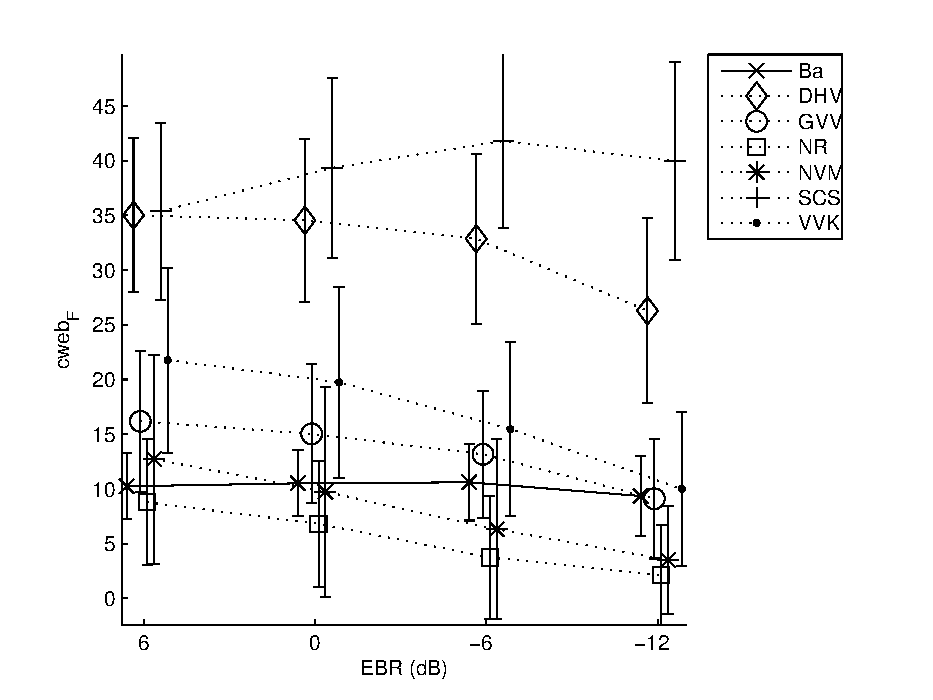
\includegraphics[width=1\textwidth]{gfxML/ebr}
\caption{Class wise event based F-measure (in percent) achieved by the systems on the QMUL instance datasets with varying EBR.}
\label{fig:ebr} 
\end{center}
\end{figure}

\subsubsection{Corpus IRCCYN}

\begin{table}
\begin{center} 
\begin{tabular}{lccc}
system/dataset & testQ & insI & absI \\ 
\hline 
Baseline & \textbf{9.0$\pm$4.8$^*$}  &  5.9$\pm$2.9 &  5.6$\pm$2.9 \\ 
DHV      & \textbf{30.7$\pm$8.4$^*$} & 10.0$\pm$5.8 &  9.5$\pm$5.6 \\ 
GVV      & \textbf{13.2$\pm$8.0$^*$} &  5.6$\pm$3.7 &  5.5$\pm$3.6 \\
NR       & \textbf{21.5$\pm$6.5$^*$} &  4.6$\pm$3.4 &  5.4$\pm$4.5 \\ 
NVM      & \textbf{28.2$\pm$5.9$^*$} &  3.1$\pm$3.1 &  3.2$\pm$3.0 \\ 
SCS      & \textbf{41.5$\pm$7.6$^*$} & 35.4$\pm$7.2 & 34.0$\pm$6.7 \\ 
VVK      & \textbf{24.6$\pm$6.8$^*$} &  6.6$\pm$5.7 &  7.3$\pm$6.3 \\ 
\hline
\end{tabular} 
\end{center}  
\caption{Results of the evaluated systems on the IRCCYN datasets, compared with the \emph{test-QMUL} dataset. Results in bold are equivalent (t-test per row at 0.05 significance level) to the best performance (depicted with a $^*$).}
\label{tab:irccyn} 
\end{table} 

Quand on considère une tâche de classification, un problème de taille est de savoir si le système évalué est capable de généraliser ses capacités de classification à des données non-observées, mais qui correspondent aux classes considérées dans les corpus de \emph{train} et de \emph{development}.

Afin d'évaluer les capacités de généralisation des algorithmes, nous considérons les performances obtenus sur les corpus de scènes simulées avec la banque de donnée de sons isolés \emph{IRCCYN}, à savoir \emph{abstract-IRCCYN} et \emph{instance-IRCCYN}, dont les samples (événements et \emph{background}) ont été enregistrés dans des environnements acoustiques différents de ceux des corpus \emph{test-},  \emph{abstract-} et \emph{instance-QMUL}.

Les résultats sont affichés sur le tableau~\ref{tab:irccyn} et la figure~\ref{fig:irccyn}. Alors que la plupart des systèmes ont obtenus des performances comparables entre \emph{test-QMUL} et les corpus \emph{abstract-} et \emph{instance-QMUL}, tous algorithmes voient leurs résultats diminuer de manière significative pour les corpus  \emph{abstract-} et \emph{instance-IRCCYN}. De plus, à l'exception du système SCS, tous les systèmes ont des résultats équivalents à la \emph{baseline} pour les corpus \emph{IRCCYN}, en particulier le système DHV, qui pourtant montre de bons résultats pour les corpus \emph{QMUL}.

L'ensemble de ces résultats nous permettent de conclure que, pour les systèmes DHV, GVV, NR, NVM et VVK, le gain de performance par rapport à la baseline observé sur le corpus \emph{test-QMUL} n'est dû qu'à une sur-adaptation des systèmes aux données d'entraînement (corpus \emph{train}). 

Comme on peut clairement le voir sur la figure~\ref{fig:irccyn}, seul le système SCS (gagnant du challenge AED DCASE 2013), arrive à maintenir des performances similaires entre tous les corpus considérés. Cette capacité de généralisation est par ailleurs cohérente, le système parvenant en effet à généraliser sur des scènes dont on a fait varier: 

\begin{itemize}
\item les samples sélectionnés (en considérant deux banques de sons isolés différents);
\item les positions temporels des samples;
\item les $EBRs$.
\end{itemize}

\begin{figure}[t]
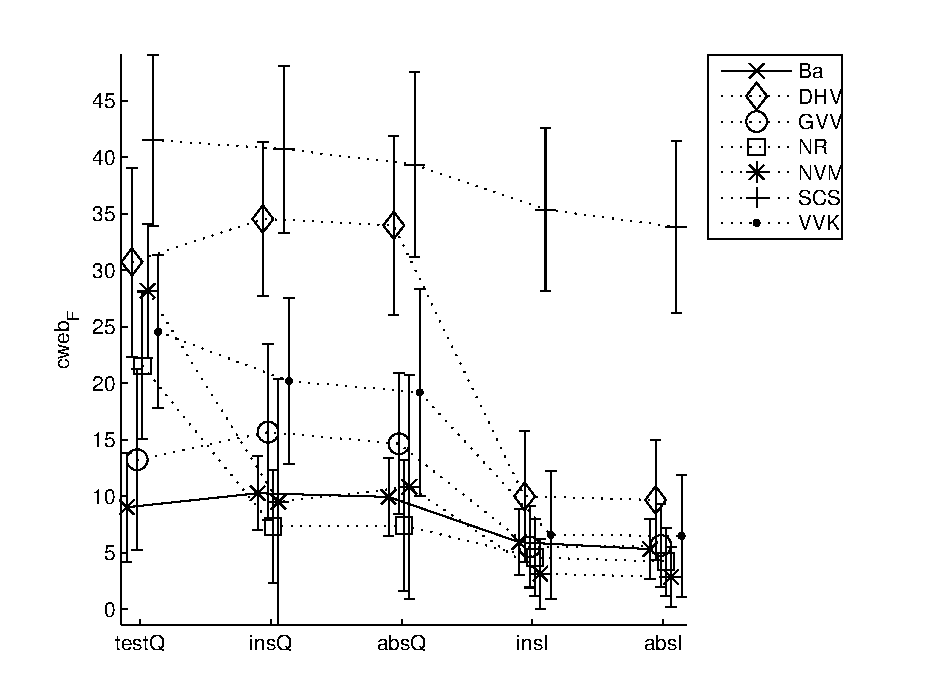
\includegraphics[width=1\textwidth]{gfxML/irccyn}
\caption{ Class-wise event based F-measure achived by the different systems on the QMUL and IRCCYN datasets.}
\label{fig:irccyn}
\end{figure}

\subsection{Discussion}

\gl{TODO:  To summarize the results discussed above, the use of the proposed model allows us to:}

\begin{enumerate}
\item Replicate the ranking of systems in the same recording conditions for 5 systems among 7. The two problematic systems have their performance degraded most probably because of an overfit of the discriminative classifier they used.
\item Evaluate the generalization properties of the systems in new recording conditions. In this respect, the SCS system is the only one to generalize correctly.
\item Evaluate the robustness of the systems while facing different levels of background noise. Notably, once again, the SCS system exhibits good and stable performance across the EBR range, most probably because of an effective noise removal pre-processing step.
\end{enumerate}

\gl{TODO:In light of those results, we believe that considering carefully designed simulated data is useful for gaining knowledge about the properties and behaviors of the systems under evaluation, thus helping designers in their algorithmic choices and their evaluation. Important factors influencing the performance such as the noise level, the level of polyphony, the intra-class diversity (acoustical difference between training and testing data) can be evaluated independently, without the burden of experimentally recording data with the desired properties and manually annotating them.}

\gl{Even though the sole use of synthetic data for validating a computational approach is clearly not sufficient, we believe that the sole use of real data may not be sufficient either, should one wish to gain knowledge about the impact of some design and parametrization issues involved in the implementation of an engineering system. Indeed, real data is most of the time a scarce resource as the careful design of a large evaluation dataset is a very demanding task. Moreover, an a posteriori annotation of the presence of the events has to be performed by several humans whose agreement is not perfect and has to be mitigated.}

\gl{We thus believe that considering simulated data is an in between approach, that together with final validation using real data is useful to get a better understanding about the systems under evaluation. The simulated sound scene datasets have been generated using a dedicated set of Matlab functions, which are publicly available\footnote{https://bitbucket.org/mlagrange/simscene/downloads}.}

\section{Le challenge DCASE  2016}

\subsection{Objectifs}

\subsection{Génération des corpus}

\subsection{Planification expérimentale}

\subsection{Résultats}

\subsection{Discussion}
%*****************************************
%*****************************************
%*****************************************
%*****************************************
%*****************************************




